\documentclass[10pt]{article}
\usepackage[utf8]{inputenc}
\usepackage[T1]{fontenc}
\usepackage{amsmath}
\usepackage{amsfonts}
\usepackage{amssymb}
\usepackage[version=4]{mhchem}
\usepackage{stmaryrd}
\usepackage{caption}
\usepackage{multirow}
\usepackage{graphicx}
\usepackage[export]{adjustbox}
\graphicspath{ {./images/} }
\usepackage{hyperref}
\hypersetup{colorlinks=true, linkcolor=blue, filecolor=magenta, urlcolor=cyan,}
\urlstyle{same}

\title{Entrepreneurship, Frictions, and Wealth }

\author{Marco Cagetti\\
Board of Governors, Federal Reserve System\\
Mariacristina De Nardi\\
Federal Reserve Bank of Chicago, National Bureau of Economic Research, and University of Minnesota}
\date{}


%New command to display footnote whose markers will always be hidden
\let\svthefootnote\thefootnote
\newcommand\blfootnotetext[1]{%
  \let\thefootnote\relax\footnote{#1}%
  \addtocounter{footnote}{-1}%
  \let\thefootnote\svthefootnote%
}

%Overriding the \footnotetext command to hide the marker if its value is `0`
\let\svfootnotetext\footnotetext
\renewcommand\footnotetext[2][?]{%
  \if\relax#1\relax%
    \ifnum\value{footnote}=0\blfootnotetext{#2}\else\svfootnotetext{#2}\fi%
  \else%
    \if?#1\ifnum\value{footnote}=0\blfootnotetext{#2}\else\svfootnotetext{#2}\fi%
    \else\svfootnotetext[#1]{#2}\fi%
  \fi
}

\begin{document}
\maketitle
\captionsetup{singlelinecheck=false}


\begin{abstract}
This paper constructs and calibrates a parsimonious model of occupational choice that allows for entrepreneurial entry, exit, and investment decisions in the presence of borrowing constraints. The model fits very well a number of empirical observations, including the observed wealth distribution for entrepreneurs and workers. At the aggregate level, more restrictive borrowing constraints generate less wealth concentration and reduce average firm size, aggregate capital, and the fraction of entrepreneurs. Voluntary bequests allow some high-ability workers to establish or enlarge an entrepreneurial activity. With accidental bequests only, there would be fewer very large firms and less aggregate capital and wealth concentration.
\end{abstract}

\section*{I. Introduction}
Although many empirical studies argue that potential and existing entrepreneurs face borrowing constraints, so far there has been little

\footnotetext{We are grateful to Gadi Barlevy, Marco Bassetto, Francisco Buera, Jeff Campbell, V. V. Chari, Narayana Kocherlakota, Per Krusell, Ellen McGrattan, Kulwant Rai, Víctor RíosRull, Emmanuel Saez, Nancy Stokey, Jenni Schoppers, Kjetil Storesletten, four anonymous referees, and many seminar participants for helpful comments. We gratefully acknowledge financial support from National Science Foundation grants SES-0317872 and SES-0318014. De Nardi thanks the University of Minnesota Grant-in-Aid and Marco Cagetti the Bankard Fund for Political Economy for funding. The views herein are those of the authors and not necessarily those of the Federal Reserve Bank of Chicago, the Federal Reserve Board, the Federal Reserve System, or the National Science Foundation.
}
work on how these constraints affect aggregate capital accumulation and wealth inequality through entrepreneurial choices. Do these financial constraints hamper aggregate capital accumulation and, if so, how big is this effect? What effect do these constraints have on wealth inequality: do they exacerbate it or mitigate it? These are potentially important forces to understand the consequences of policy reforms that affect the tightness of these borrowing constraints, such as changes in the leniency of bankruptcy laws and in the degree of enforcement of property rights.

In this paper we analyze the role of borrowing constraints as determinants of entrepreneurial decisions (entry, continuation, investment, and saving), and their effects on wealth inequality and aggregate capital accumulation, in a framework that matches the observed wealth inequality very closely. In the presence of borrowing constraints, the decision to invest, the fraction of entrepreneurs, and the size distribution of firms depend on the distribution of assets in the economy. Because of this interaction, it is key to perform such an analysis in a model that matches well the extreme concentration of wealth observed in the data.

We find that more restrictive borrowing constraints generate less inequality in wealth holdings but also reduce average firm size, the number of people engaging in entrepreneurial activities, and aggregate capital accumulation. Our results also indicate that voluntary bequests are an important channel allowing some high-ability workers to establish or enlarge an entrepreneurial activity. If there were only accidental bequests, there would be fewer very large firms and less aggregate capital, but also less wealth concentration.

These findings are based on a quantitative life cycle model with altruism across generations and entrepreneurial choice, in an environment in which debt repayment cannot be perfectly enforced. The amount that entrepreneurs can borrow depends on their observable characteristics, and the entrepreneurs' assets act as collateral for their debts. Since the implicit rate of return for entrepreneurs is higher than the rate for workers, entrepreneurs have a higher saving rate, which is consistent with the data. We calibrate the parameters of the model to match key moments of the data and discuss the implications of the model and its components for entrepreneurial choice and wealth inequality. We show that our model with entrepreneurial choice matches very well the observed distribution of wealth, for both entrepreneurs and nonentrepreneurs.

This paper is related to the quantitative literature on wealth inequality. (See Cagetti and De Nardi [2005] for a comprehensive survey.) The most closely related works are the ones by De Nardi (2004), Quadrini (2000), and Castañeda, Díaz-Giménez, and Ríos-Rull (2003).

De Nardi (2004) evaluates the importance of bequest motives and intergenerational transmission of ability to explain wealth dispersion in a life cycle model and shows that a realistically calibrated bequest motive can raise wealth concentration and bring it closer to the observed data. Her model does not allow for entrepreneurial choice and falls short of explaining the extreme concentration of wealth in the hands of the richest 1 percent of the population.

Quadrini (2000) shows that a model that incorporates individualspecific technologies (entrepreneurs) and financial frictions can generate more wealth inequality than that implied by a precautionary motive, for a given process of individual ability, or "labor" income. His model relies on exogenous stochastic processes for both entrepreneurial ability and the scale of the project. We improve on Quadrini's framework by using a very parsimonious model and by allowing for endogenous choice of the amount of capital invested by the entrepreneur in the firm. We also study how financial frictions and channels affecting the intergenerational transmission of wealth affect wealth inequality and aggregate output.

Castañeda et al. (2003) adopt a dynastic model with idiosyncratic shocks and reconstruct an exogenous labor income process (which also includes most of business income) that matches earnings and wealth dispersion. The resulting labor and entrepreneurial income process implies very large earnings risk for the highest-income earners. This large risk associated with high-income realizations is the driving force that, in their framework, generates a large saving rate for the richer households, which is the fundamental mechanism driving the extreme amount of wealth observed in the hands of the richest few. In contrast to Castañeda et al., we endogenize and model explicitly the entrepreneur's investment decision and hence entrepreneurial income. In our framework the main driving force that allows the model to match the observed wealth inequality is given by potentially high rates of return from entrepreneurial investment coupled with borrowing constraints, or the observation that one needs money to make money.

Section II first documents the relationship between wealth and entrepreneurship and then surveys the evidence that entrepreneurs are borrowing constrained. Section III describes the model and our calibration procedure. Section IV discusses the role of entrepreneurship and voluntary bequests in generating large wealth concentration and studies the aggregate effects of changing the borrowing constraints. Section V inspects further the mechanisms at work in our model and compares their observable implications to those in the observed data. Section VI presents conclusions.

\section*{II. Wealth, Entrepreneurship, and Borrowing Constraints}
We first document the relationship between wealth and entrepreneurship, and we then survey the empirical evidence on the effects of borrowing constraints on entrepreneurial choice. ${ }^{1}$

\section*{A. Which Are the Rich Households?}
Wealth holdings are massively concentrated in the hands of a small fraction of households, and this wealth concentration is much larger than the one documented for labor earnings and total income. This observation raises the question of which saving motives generate the amplification in the concentration of wealth with respect to the one in income.

When one is looking at the data, it is clear that there is a tight relationship between being an "entrepreneur" and being rich. We begin by documenting this relationship, using different definitions of entrepreneurship, and we then discuss alternative ways of acquiring wealth.

The SCF asks several questions that we can use to classify a household by its occupational status:

\begin{enumerate}
  \item "Do you work for someone else, are you self-employed, or what?"
  \item "Do you (and your family living here) own or share ownership in any privately held businesses, farms, professional practices or partnerships?"
  \item "Do you (or anyone in your family living here) have an active management role in any of these businesses?"
\end{enumerate}

Table $1^{2}$ shows the fraction of people in a given occupation and the total fraction of aggregate net worth that they hold. The first line refers to people who declare that they either are business owners or are selfemployed (i.e., who answer yes to either question 1 or 2 ). This group makes up about 17 percent of the population and owns more than half of the total net worth. The second line refers to all households that own privately held businesses but do not necessarily manage them (i.e., who answer yes to question 2), and the third one focuses on the business

\footnotetext{${ }^{1}$ Whenever possible we use data from the Survey of Consumer Finances (SCF). Unlike other data sets, the SCF oversamples rich households and thus provides important advantages. First, it gives a better picture of the concentration of wealth and of the asset holdings of richer households, which include a large share of entrepreneurs. Second, as shown by Curtin, Juster, and Morgan (1989), the total wealth implied by the SCF is very close to the total wealth implied by aggregate data; the SCF can thus be used to calibrate aggregates (e.g., the share of entrepreneurial wealth and the percentage of entrepreneurs) in a general equilibrium model such as the one developed in this paper.\\
${ }^{2}$ All the statistics that we report here use data from the 1989 wave of the SCF. The data for the 1992 and 1995 waves are similar. The results are available from the authors on request.
}\begin{table}[h]
\begin{center}
\captionsetup{labelformat=empty}
\caption{TABLE 1\\
Percentage of Entrepreneurs (According to Various Definitions) in the Population and Corresponding Share of Total Wealth Held}
\begin{tabular}{|l|l|l|}
\hline
 & Percent in Population & Share of Total Wealth \\
\hline
Business owners or self-employed & 16.7 & 52.9 \\
\hline
All business owners & 13.3 & 48.8 \\
\hline
Active business owners & 11.5 & 41.6 \\
\hline
All self-employed & 11.1 & 39.0 \\
\hline
Self-employed business owners & 7.6 & 33.0 \\
\hline
\end{tabular}
\end{center}
\end{table}

owners who effectively manage their own business(es) (i.e., who answer yes to question 3). The fourth line refers to those who report being selfemployed (yes to question 1) and the fifth line to those who both are self-employed and are business owners with an active management role (yes to questions 1, 2, and 3). The self-employed business owners are 7.6 percent of the population and yet hold 33 percent of the total net worth. The key message of this table is that, regardless of the specific definition of entrepreneurship used, entrepreneurs are a relatively small fraction of the population and hold a large fraction of the total net worth.

Table 2 documents wealth concentration in the United States: the households in the top 1 percent of the wealth distribution hold about 30 percent of total net worth, and those in the top 5 percent hold more than half of the total. Table 3 reports the fraction of various definitions of entrepreneurs in the corresponding wealth quantile of the overall wealth distribution. A whopping 81 percent of those who belong to the top 1 percent of the wealth distribution declare that they either are selfemployed or are business owners. All business owners are 76 percent of the richest 1 percent of households, and the fraction of the business owners who actively manage their own business(es) is 65 percent; hence some of the business owners are "investors" who own a business that is managed and run by someone else. The self-employed make up 62 percent of the households in the top 1 percent of the wealth distribution, and the self-employed business owners are 54 percent. The overall message of this table is that most rich people are entrepreneurs.

Table 4 reports mean and median asset holdings by occupational

\begin{table}[h]
\begin{center}
\captionsetup{labelformat=empty}
\caption{TABLE 2\\
U.S. Wealth Distribution}
\begin{tabular}{lcccc}
\hline\hline
 & \multicolumn{4}{c}{Fraction of People, Top} \\
\cline { 2 - 5 }
 & $1 \%$ & $5 \%$ & $10 \%$ & $20 \%$ \\
\hline
Total net worth held & $30 \%$ & $54 \%$ & $67 \%$ & $81 \%$ \\
\hline
\end{tabular}
\end{center}
\end{table}

\begin{table}[h]
\begin{center}
\captionsetup{labelformat=empty}
\caption{TABLE 3\\
Fraction (\%) of Entrepreneurs (According to Various Definitions) in a Given Wealth Percentile of the Overall U.S. Wealth Distribution}
\begin{tabular}{|l|l|l|l|l|}
\hline
\multirow{2}{*}{} & \multicolumn{4}{|c|}{Wealth Percentile, Top} \\
\hline
 & 1\% & 5\% & 10\% & 20\% \\
\hline
Business owners or self-employed & 81 & 68 & 54 & 39 \\
\hline
All business owners & 76 & 62 & 49 & 36 \\
\hline
Active business owners & 65 & 51 & 42 & 30 \\
\hline
Self-employed & 62 & 47 & 38 & 26 \\
\hline
Self-employed business owners & 54 & 39 & 32 & 22 \\
\hline
\end{tabular}
\end{center}
\end{table}

\begin{table}[h]
\begin{center}
\captionsetup{labelformat=empty}
\caption{TABLE 4\\
Median and Mean Net Worth (in Thousands of Dollars) for Various Groups of People}
\begin{tabular}{|l|l|l|}
\hline
 & Median & Mean \\
\hline
Whole population & 47 & 189 \\
\hline
Business owners or self-employed & 172 & 599 \\
\hline
All business owners & 205 & 695 \\
\hline
Business owners but not active management & 293 & 768 \\
\hline
Business owners not selfemployed & 179 & 470 \\
\hline
All self-employed & 169 & 665 \\
\hline
Self-employed (active) business owners & 265 & 829 \\
\hline
Self-employed and not business owners & 36 & 224 \\
\hline
\end{tabular}
\end{center}
\end{table}

status. Regardless of the specific definition of entrepreneurship, entrepreneurs are much richer than nonentrepreneurs. The business owners, however, tend to be richer than the self-employed. Not surprisingly, the poorest are those who declare being self-employed but not business owners; some of these households might be the low-wage workers who turn to self-employment for lack of better opportunities ${ }^{3}$ or people who are self-employed as a hobby. Interestingly, the business owners who do not have an active management role in the business are very rich and are likely to use the business as an investment opportunity.

We have seen that many of the rich people are entrepreneurs. But who are the others, and how did they become rich? Unfortunately, the SCF provides only very coarse classifications by occupation, for example,

\footnotetext{${ }^{3}$ Rissman (2003) documents that in the National Longitudinal Survey of Youth, more than one-quarter of all younger men experience some period of self-employment, and many of them return to wage work. She argues that for these workers self-employment is a low-income alternative to wage work and provides an alternative source of income for unemployed workers. Rissman also finds that young men are more likely to become selfemployed when their wage opportunities are more limited, as in periods of economic downturns.
}
lumping together managers, professionals, singers, performers, and so forth and thus provides very little data to answer this question. The other nationally representative samples miss the very rich. We study the Forbes magazine list of the 400 richest people in the United States. While this is a very restricted sample, it certainly focuses on the rich. According to this data set, of the 400 wealthiest American people in various years, 61-80 percent were self-made (typically by individuals who started a firm), whereas the rest inherited the family's fortune, which was typically originated by one or more businesses started by one of their parents or grandparents. ${ }^{4}$ Extremely few entries in this list were people such as entertainers or athletes who acquired their wealth through high incomes without starting as entrepreneurs. By cross-comparing the 2004 list with the one for the top 100 "celebrities" for the same year (also compiled by Forbes), we find that only three of the top 100 celebrities make it to the list of the top 400 richest Americans: George Lucas, Oprah Winfrey, and Steven Spielberg. Interestingly, Spielberg put up $\$ 33$ million for 22 percent of his upstart studio in 1994 and thus used a significant amount of his own money to start his empire.

\section*{B. Entrepreneurship and Borrowing Constraints}
To estimate the severity of borrowing constraints on entrepreneurial entry and continuation decisions, one would want to know how much potential and existing entrepreneurs would like to borrow, at what interest rate, and how much they are actually able to borrow, and at what price. Unfortunately, such data are not available.

Many papers have used a variety of data sets and methodologies to indirectly estimate the severity of borrowing constraints for entrepreneurs. Among these works, Evans and Jovanovic (1989) and Buera (2006) estimate structural models of entrepreneurship and find evidence of borrowing constraints; Gentry and Hubbard (2004) and Eisfeldt and Rampini (2005) also argue that costly external financing has important implications for investment and saving decisions. Holtz-Eakin, Joulfaian, and Rosen (1994) study the effects of receiving a bequest on both potential and existing entrepreneurs. They find that the receipt of a bequest (and thus an increase in wealth) increases the probability of starting a business. They also find that existing sole-proprietors who receive a bequest not only are more likely to stay in business but also experience a substantial increase in the enterprise's receipts.

More recently, Hurst and Lusardi (2004) have disputed the relevance

\footnotetext{${ }^{4}$ The fraction of heirs in the Forbes 400 list was 39 percent in 2004 (our computations), whereas it varies between 20 percent and 30 percent in other years according to Smith (2001). This fraction is quite volatile because of the small sample size of this list.
}
of borrowing constraints to entrepreneurial entry. They estimate that the probability of entering entrepreneurship as a function of initial wealth is first flat over a large range of the wealth distribution, and it then increases for the richest workers. We will show that a model of entrepreneurial choice with borrowing constraints is capable of generating this type of entry probabilities as a function of one's own wealth. We will also discuss that the lack of borrowing constraints on entrepreneurial entry does not imply lack of borrowing constraints on entrepreneurial investment after entry.

The need to accumulate assets in the presence of borrowing constraints may also generate high saving rates among entrepreneurs (or households planning to become entrepreneurs). Using different data sets, Quadrini (1999) and Gentry and Hubbard (2004) show higher saving rates for entrepreneurs than for the rest of the population, and Buera (2006) shows higher saving rates also in the years before entry into entrepreneurship.

To provide more evidence on the existence of borrowing constraints, we also look at the data on entrepreneurs using their collateral for their business and on entrepreneurs declaring that they have been turned down for credit or that they did not apply for credit because they thought that they would be turned down.

The SCF asks explicitly about whether some of the debts are explicitly collateralized with the entrepreneur's own private assets. These numbers are just an indication because they include the use of only personal assets (other than the business itself) and do not indicate the relation between the amount borrowed and the size of the business, nor the amount of borrowing desired by the entrepreneur. Among the selfemployed business owners, 29 percent declare that they currently use their own personal assets as collateral to finance their business. Within this group, the median ratio of personal collateral to business value is 21 percent, for the top decile is 77 percent, and for the top 5 percent is 100 percent. These fractions do not change significantly across quantiles of the wealth distribution, thus suggesting that many businesses do need to put up collateral in order to borrow, regardless of their size.

Among the self-employed business owners, 18 percent report that they have been turned down for credit, and 9 percent state that they thought of applying but changed their mind because they thought they might be turned down.

The severity of borrowing constraints potentially depends on bankruptcy laws. Berkowitz and White (2004) show that the higher exemption levels on personal bankruptcy, the higher the probability of being denied credit and the smaller the amount of loans made. This suggests that higher exemptions lower the incentive to repay and thus generate more stringent borrowing constraints.

\section*{III. The Model}
\section*{A. Demographics}
We adopt a life cycle model with intergenerational altruism. To make the results quantitatively interesting, we need short time periods. To make the model computationally manageable, we have to keep the number of stages of life small. To reconcile these two necessities, we adopt a modeling device introduced by Blanchard (1985) and generalized by Gertler (1999) to a life cycle setting.

Households go through two stages of life, young and old age. A young person faces a constant probability of aging during each period ( $1- \pi_{y}$ ), and an old person faces a constant probability of dying during each period ( $1-\pi_{o}$ ). When an old person dies, his offspring enters the model, carrying the assets bequeathed to him by the parent. Appropriately parameterized, this framework generates households for which the average lengths of the working period and the retirement period are realistic. Our model period is one year.

There is a continuum of households of measure one. The households are subject to idiosyncratic shocks, but there is no aggregate uncertainty, as in Bewley (1977).

\section*{B. Preferences}
The household's utility from consumption is given by $c^{1-\sigma} /(1-\sigma)$. The households discount the future at rate $\beta$, and, in addition, they discount the utility of their offspring at rate $\eta$.

To study the role of bequests, our model nests life cycle and fully altruistic households as two extreme cases. In the purely life cycle version of the model, individuals put no weight on the utility of their descendants ( $\eta=0$ ). In the perfectly altruistic version, individuals care about their descendants as much as themselves ( $\eta=1$ ). We assume exogenous labor supply.

\section*{C. Technology}
Each person possesses two types of ability, which we take to be exogenous, stochastic, positively correlated over time, and uncorrelated with each other. Entrepreneurial ability ( $\theta$ ) is the capacity to invest capital more or less productively. Working ability ( $y$ ) is the capacity to produce income out of labor.

Entrepreneurs can borrow and invest capital in a technology whose return depends on their own entrepreneurial ability: those with higher ability levels have higher average and marginal returns from capital. When the entrepreneur invests $k$, the production is given by $\theta k^{\nu}$, where\\
$\nu \in[0,1]$. Entrepreneurs thus face decreasing returns from investment, since their managerial skills become gradually stretched over larger and larger projects (as in Lucas [1978]). Hence, while entrepreneurial ability is exogenously given, the entrepreneurial rate of return from investing in capital is endogenous and is a function of the size of the project that the entrepreneur implements.

There is no within-period uncertainty regarding the returns of the entrepreneurial project. The ability $\theta$ is observable and known by all at the beginning of the period. We therefore ignore problems arising both from partial observability and costly state verification and from diversification of entrepreneurial risk. The simplification is adopted to focus only on the effect of the borrowing constraint.

Workers can save (but not borrow) at a riskless, constant rate of return.\\
Many firms are not controlled by a single entrepreneur and are not likely to face the same financing restrictions that we stress in our model. Therefore, as in Quadrini (2000), we model two sectors of production: one populated by the entrepreneurs and one by "nonentrepreneurial" firms. The nonentrepreneurial sector is represented by a standard CobbDouglas production function:


\begin{equation*}
F\left(K_{c}, L_{c}\right)=A K_{c}^{\alpha} L_{c}^{1-\alpha} \tag{1}
\end{equation*}


where $K_{c}$ and $L_{c}$ are the total capital and labor inputs in the nonentrepreneurial sector and $A$ is a constant. In both sectors, capital depreciates at a rate $\delta$.

\section*{D. Credit Market Constraints}
As in Marcet and Marimon (1992), Kehoe and Levine (1993), Albuquerque and Hopenhayn (2004), and Cooley, Marimon, and Quadrini (2004), the borrowing constraints are endogenously determined in equilibrium and stem from the assumption that contracts are imperfectly enforceable.

Imperfect enforceability of contracts means that the creditors will not be able to force the debtors to fully repay their debts as promised and that the debtors fully repay only if it is in their own interest to do so. Since both parties are aware of this feature and act rationally, the lender will lend to a given borrower only an amount (possibly zero) that will be in the debtor's interest to repay as promised.

In particular, we assume that the entrepreneurs who borrow can either invest the money and repay their debt at the end of the period or run away without investing it and be workers for one period. In the latter case, they retain a fraction $f$ of their working capital $k$ (which includes their own assets and borrowed money), and their creditors seize the rest.

In the absence of market imperfections, the optimal level of capital is only related to technological parameters and does not depend on initial assets. In our framework, instead, the higher the amount of an entrepreneur's own wealth invested in the business, the larger the amount that the entrepreneur would lose in case of default, the lower the temptation to default, and the larger the sum that the creditor is willing to lend to the entrepreneur. Hence, the entrepreneur's assets act as collateral, although the loan need not be fully collateralized.

As a result, not all potentially profitable projects receive appropriate funding. Households with little wealth can borrow little, even if they have high ability as entrepreneurs. Since the entrepreneur forgoes his potential earnings as a worker, he will choose to become an entrepreneur only if the size of the firm that he can start is big enough; that is, he is rich enough to be able to borrow and invest a suitable amount of money in his firm.

\section*{E. Households}
At the beginning of each period, before any economic decisions are made, the current ability levels are known with certainty, whereas next period's levels are uncertain.

Each young individual starts the period with assets $a$, entrepreneurial ability $\theta$, and worker ability $y$ and chooses whether to be an entrepreneur or a worker during the current period.

An old entrepreneur can decide to keep the activity going or to retire, and a retiree cannot start a new entrepreneurial activity. We allow entrepreneurs to remain active when old to capture the fact that, while most workers retire before age 65, entrepreneurs often continue their activity until much later.

\section*{The Young's Problem}
The young's state variables are his current assets $a$, working ability $y$, and entrepreneurial ability $\theta$. His value function is


\begin{equation*}
V(a, y, \theta)=\max \left\{V_{e}(a, y, \theta), V_{w}(a, y, \theta)\right\} \tag{2}
\end{equation*}


where $V_{e}(a, y, \theta)$ is the value function of a young individual who manages an entrepreneurial activity during the current period. In order to invest $k$, the young entrepreneur borrows $k-a$ from a financial intermediary at the interest rate $r$, which is the risk-free interest rate at which people can borrow and lend in this economy. Consumption $c$ is enjoyed at the\\
end of the period. We have


\begin{gather*}
V_{e}(a, y, \theta)=\max _{c, k, a^{\prime}}\left\{u(c)+\beta \pi_{y} E V\left(a^{\prime}, y^{\prime}, \theta^{\prime}\right)+\beta\left(1-\pi_{y}\right) E W\left(a^{\prime}, \theta^{\prime}\right)\right\},  \tag{3}\\
a^{\prime}=(1-\delta) k+\theta k^{\nu}-(1+r)(k-a)-c,  \tag{4}\\
u(c)+\beta \pi_{y} E V\left(a^{\prime}, y^{\prime}, \theta^{\prime}\right)+\beta\left(1-\pi_{y}\right) E W\left(a^{\prime}, \theta^{\prime}\right) \geq V_{w}(f \cdot k, y, \theta),  \tag{5}\\
a \geq 0, \tag{6}
\end{gather*}


and


\begin{equation*}
k \geq 0 . \tag{7}
\end{equation*}


The expected value of the value function is taken with respect to ( $y^{\prime}$, $\theta^{\prime}$ ), conditional on ( $y, \theta$ ); $F\left(y^{\prime}, \theta^{\prime} \mid y, \theta\right)$ is a first-order Markov process; and $W\left(a^{\prime}, \theta^{\prime}\right)$ is the value function of the old entrepreneur at the beginning of the period, before he has decided whether he wants to stay in business or retire.

The function $V_{w}(a, y, \theta)$ is the value function for the young who chooses to be a worker during the current period. We have


\begin{equation*}
V_{w}(a, y, \theta)=\max _{c, a^{\prime}}\left\{u(c)+\beta \pi_{y} E V\left(a^{\prime}, y^{\prime}, \theta^{\prime}\right)+\beta\left(1-\pi_{y}\right) W_{r}\left(a^{\prime}\right)\right\} \tag{8}
\end{equation*}


subject to equation (6) and


\begin{equation*}
a^{\prime}=(1+r) a+(1-\tau) w y-c, \tag{9}
\end{equation*}


where $w$ is the wage and $\tau$ is a proportional payroll tax used to finance old-age social security. We explicitly model old-age social security because it is a very important program affecting life cycle saving decisions.

When the worker becomes old, he retires, and $W_{r}\left(a^{\prime}\right)$ is the corresponding value function.

\section*{The Old's Problem}
The old entrepreneur can choose to continue the entrepreneurial activity or to retire. The old person's state variables are therefore his current assets $a$, his entrepreneurial ability $\theta$, and whether he was a retiree or an entrepreneur during the previous period.

The value function of an old entrepreneur is


\begin{equation*}
W(a, \theta)=\max \left\{W_{e}(a, \theta), W_{r}(a)\right\} \tag{10}
\end{equation*}


where $W_{e}(a, \theta)$ is the value function for the old entrepreneur who stays in business, and $W_{r}(a)$ is the value function of the old, retired person.

We denote by $\eta$ the weight on the utility of the descendants. If $\eta=$ 0 , the household behaves as a pure life cycle; if $\eta=1$, the household behaves as a dynasty. We have


\begin{equation*}
W_{e}(a, \theta)=\max _{c, k, a^{\prime}}\left\{u(c)+\beta \pi_{o} E W\left(a^{\prime}, \theta^{\prime}\right)+\eta \beta\left(1-\pi_{o}\right) E V\left(a^{\prime}, y^{\prime}, \theta^{\prime}\right)\right\} \tag{11}
\end{equation*}


subject to equations (4), (6), and (7) and


\begin{equation*}
u(c)+\beta \pi_{o} E W\left(a^{\prime}, \theta^{\prime}\right)+\eta \beta\left(1-\pi_{o}\right) E V\left(a^{\prime}, y^{\prime}, \theta^{\prime}\right) \geq W_{r}(f \cdot k) \tag{12}
\end{equation*}


The offspring of an entrepreneur is born with ability level $\left(\theta^{\prime}, y^{\prime}\right)$. The expected value of the offspring's value function with respect to $y^{\prime}$ is computed using the invariant distribution of $y$, whereas the one with respect to $\theta^{\prime}$ is conditional on the parent's $\theta$ and evolves according to the same Markov process that each person faces for $\theta$ while alive. This is justified by the assumption that the offspring of an entrepreneur inherits the parent's firm.

A retired person (who is not an entrepreneur) receives pensions and social security payments ( $p$ ) and consumes his assets. His value function is


\begin{equation*}
W_{r}(a)=\max _{c, a^{\prime}}\left\{u(c)+\beta \pi_{o} W_{r}\left(a^{\prime}\right)+\eta \beta\left(1-\pi_{o}\right) E V\left(a^{\prime}, y^{\prime}, \theta^{\prime}\right)\right\} \tag{13}
\end{equation*}


subject to equation (6) and


\begin{equation*}
a^{\prime}=(1+r) a+p-c \tag{14}
\end{equation*}


The expected value of the child's value function is taken with respect to the invariant distribution of $y$ and $\theta$.

\section*{F. Equilibrium}
Let $\boldsymbol{x}=(a, y, \theta, s)$ be the state vector for an individual in our economy, where $s$ distinguishes young workers, young entrepreneurs, old entrepreneurs, and old retired. From the decision rules that solve the maximization problem and the exogenous Markov process for income and entrepreneurial ability, we can derive a transition function that provides the probability distribution of $\boldsymbol{x}^{\prime}$ (the state next period) conditional on $\boldsymbol{x}$.

A stationary equilibrium is given by a risk-free interest rate $r$, wage rate $w$, and tax rate $\tau$; allocations $c(\boldsymbol{x}), a(\boldsymbol{x})$, occupational choices, and investments $k(\boldsymbol{x})$; and a constant distribution of people over the state variables $\boldsymbol{x}, m^{*}(\boldsymbol{x})$, such that, given $r, w$, and $\tau$, the following conditions hold:

\begin{itemize}
  \item The functions $c, a$, and $k$ solve the maximization problems described above.
  \item The capital and labor markets clear. Entrepreneurs use their own labor. The total labor supplied by the workers equals the total labor employed in the nonentrepreneurial sector. The total savings in the economy equal the sum of the total capital employed in the nonentrepreneurial and in the entrepreneurial sectors.
  \item The wage and interest rates are given by the marginal products of each factor of production, and the rate of return from investing in capital in the nonentrepreneurial sector must equate the riskfree rate that equates savings and investment.
  \item The social security budget constraint is balanced period by period: $\tau$ is chosen so that total labor income taxes equal total old-age social security payments.
  \item The distribution $m^{*}$ is the invariant distribution for the economy.
\end{itemize}

Appendix B outlines the algorithm that we use to solve the model.

\section*{G. Calibration}
The empirical definition of entrepreneurship that we use for the calibration must be consistent with the notion of entrepreneur in our framework. In our model an entrepreneur runs his own business, invests his own wealth in it, has a potentially high return from investing in his business, and faces borrowing constraints to starting or expanding his firm. Our entrepreneur is not simply a manager in a firm, is not an "investor" (who does not have a key role in managing the firm), and is not a person working on his own because he is virtually unemployable in any other firm. For this reason we use the SCF data to classify as entrepreneurs the households that declare that they are self-employed, that they do own a business (or a share of one), and that they have an active management role in it. Our definition thus eliminates managers (who are not likely to think of themselves as self-employed) and the business owners who do not manage the business that they own. It is thus likely to eliminate (at least part of) "reverse causation": for example, people who are rich and acquire a business for investment or as a hobby but do not have an active management role in it. By taking the intersection of the self-employed and the active business owners, our definition is also likely to eliminate the self-employed households that either mostly invest their (possibly considerable) human capital in the business, but very little physical capital, or are self-employed only because their wage opportunities are very poor. Although for different reasons, none of these households are entrepreneurs in the sense of our model, nor are they likely to be borrowing constrained from starting a profitable business.

Our general calibration strategy is to reduce the number of param-

\begin{table}[h]
\begin{center}
\captionsetup{labelformat=empty}
\caption{TABLE 5\\
Parameters of the Model}
\begin{tabular}{|l|l|l|}
\hline
 & Value & Source(s) \\
\hline
\multirow[b]{2}{*}{$\sigma$} & \multicolumn{2}{|c|}{A. Fixed Parameters} \\
\hline
 & 1.5 & Attanasio et al. (1999) \\
\hline
$\delta$ & . 06 & Stokey and Rebelo (1995) \\
\hline
$\alpha$ & . 33 & Gollin (2002) \\
\hline
A & 1.0 & Normalization \\
\hline
$\pi_{y}$ & . 978 & See text \\
\hline
$\pi_{o}$ & . 911 & See text \\
\hline
$\mathbf{P}_{y}$ & See text & Storesletten et al. (2004) \\
\hline
$p$ & 40\% of average yearly income & Kotlikoff et al. (1999) \\
\hline
$\eta$ & 1.0 & Perfect altruism \\
\hline
 &  &  \\
\hline
$\beta$ & . 865 &  \\
\hline
$\theta$ & [0, .51] &  \\
\hline
$\mathbf{P}_{\theta}$ & See text &  \\
\hline
$\nu$ & . 88 &  \\
\hline
$f$ & 75\% &  \\
\hline
\end{tabular}
\end{center}
\end{table}

eters that we use to match the data as much as possible. We thus divide our parameters into two sets. The first set of parameters either can be easily estimated from the data without using our model (e.g., the length of young and old age) or has been estimated by many previous studies (e.g., risk aversion). We use the second set of parameters to match some relevant moments of the data.

Table 5 lists the parameters of the model. Panel A of the table shows the set of parameters that we take from other studies and do not use to match moments of the data.

We take the coefficient of relative risk aversion to be 1.5, a value close to those estimated by, among others, Attanasio et al. (1999). As is standard in the business cycle literature, we choose a depreciation rate $\delta$ of 6 percent. The share of income that goes to capital in the nonentrepreneurial sector is 0.33 , and the scaling factor $A$ is normalized to one. The probabilities of aging and of death are such that the average length of the working life is 45 years, and the average length of the retirement period is 11 years. The logarithm of the income process $y$ for working people is assumed to follow an $\operatorname{AR}(1)$. We take its persistence to be 0.95 , as estimated by Storesletten, Telmer, and Yaron (2004). The variance is chosen to match the Gini coefficient for earnings of 0.38, the average found in the Panel Study of Income Dynamics (PSID). The matrix $\mathbf{P}_{y}$ is a transition matrix for the discretized labor income process. We assume that the income and the entrepreneurial ability processes evolve independently. (See App. A for exact values of the income and ability\\
processes and a discussion of the effects of assuming positive correlation between entrepreneurial and working abilities.) The social security replacement rate is 40 percent of average income, net of taxes (see Kotlikoff, Smetters, and Walliser 1999). In the baseline case we set $\eta=1$ (perfect altruism) and then study the no-altruism case.

Panel B of table 5 lists the remaining parameters of the model: $\beta$, the vector $\boldsymbol{\theta}, \mathbf{P}_{\theta}, \nu$, and $f$ and their corresponding values in the baseline calibration. We consider a very parsimonious calibration and allow for only two values of entrepreneurial ability: zero (no entrepreneurial ability) and a positive number. This implies that the transition matrix $\mathbf{P}_{\theta}$ is a $2 \times 2$ matrix. Since its rows have to sum to one, this gives us two parameters to calibrate, corresponding to the persistence of each of the two ability states (see App. A for the actual values used). We also have to choose values for $\nu$, the degree of decreasing returns to scale to entrepreneurial ability, and $f$, the fraction of working capital the entrepreneur can keep in case he defaults. This gives us a total of six parameters to calibrate to the data. ${ }^{5}$

We use these six parameters to pin down the following moments generated by the model: the capital-output ratio, the fraction of entrepreneurs in the population, the fraction of entrepreneurs exiting entrepreneurship during each period, the fraction of workers becoming entrepreneurs during each period, ${ }^{6}$ the ratio of median net worth of entrepreneurs to that of workers, and the wealth Gini coefficient. It should be noted that the Gini coefficient is just a summary of wealth inequality. A model can match the Gini coefficient for wealth while at the same time doing a very poor job of matching the overall wealth distribution. For example, a high Gini coefficient can be generated either by having too many people holding no wealth or by having just a few people holding a lot of it.

Given the features matched in the calibration, we analyze how well the model matches the overall distribution of wealth and the distributions of wealth for entrepreneurs and workers. We use the implications of the model in this respect as a check of the validity of our model. We then study the role of borrowing constraints and voluntary bequests.

\footnotetext{${ }^{5}$ Note that we do not impose an exogenous minimum firm size or investment level nor start-up costs. We experimented adding a fixed start-up cost and a minimum firm size (both on the order of $\$ 5,000-\$ 20,000$ ), but doing so had no significant impact on our numerical results.\\
${ }^{6}$ Both in the model and in the data, entry and exit rates refer only to people who were in the model (or survey) in both periods and transitioned from one occupation to the other; they do not include people who die while running an enterprise, nor people who start their enterprise at the beginning of their economic life. For this reason, entry, exit, and the steady-state fraction of entrepreneurs are not linked by the identity that would hold in an economy with infinitely lived agents.
}\begin{table}[h]
\begin{center}
\captionsetup{labelformat=empty}
\caption{TABLE 6\\
Comparing Data and Models with and without Entrepreneurs}
\begin{tabular}{|l|l|l|l|l|l|l|l|}
\hline
\multirow{2}{*}{} & \multirow[b]{2}{*}{CapitalOutput Ratio} & \multirow[b]{2}{*}{Wealth Gini} & \multirow[b]{2}{*}{Entrepreneurs} & \multicolumn{4}{|c|}{Percentage Wealth in Top} \\
\hline
 &  &  &  & 1\% & 5\% & 20\% & 40\% \\
\hline
 & 3.0 & . 8 & 7.55\% & 30 & 54 & 81 & 94 \\
\hline
U.S. data Baseline model without entrepreneurs & 3.0 & . 6 & .0\% & 4 & 20 & 58 & 95 \\
\hline
Baseline model with entrepreneurs & 3.0 & . 8 & 7.50\% & 31 & 60 & 83 & 94 \\
\hline
\end{tabular}
\end{center}
\end{table}

\section*{IV. Results}
We first study the two versions of our model (one without and one with entrepreneurs) and discuss their ability to reproduce the observed inequality in wealth. We also highlight the key intuition of the underlying saving behavior and its implications for wealth concentration.

The first row in table 6 displays the aggregate capital-output ratio and several statistics on the wealth distribution in the United States. The notion of capital that we use includes residential structures, plant, equipment, land, and consumer durables, and it implies a capital-output ratio of about 3.0 for the period 1959-92 (Auerbach and Kotlikoff 1995). (The ratio of average wealth to average income is also about 3.0.) The data pertaining to the distribution of wealth come from the 1989 SCF. The waves for other years are similar.

In the other rows of the table, we report the corresponding statistics generated by the simulations of various versions of our model economy.

\section*{A. The Model without Enterpreneurs}
The second row of table 6 refers to the model economy without entrepreneurs. In this run, we assign zero entrepreneurial ability to everyone and change the household's discount factor to match the same capitaloutput ratio. All other parameters, including the general equilibrium prices, are the same as in the benchmark economy.

These results thus refer to a model economy with labor earnings risk and a simplified life cycle structure. As we can see from the table, this model economy produces a distribution of wealth that is much less concentrated than that in the data and that, in particular, does not explain the emergence of the large estates that characterize the upper tail of the distribution of wealth. Figure 1 compares the distribution of wealth implied by the data (1989 SCF, in thousands of dollars) with the distribution of wealth implied by the model without entrepreneurial

\begin{figure}[h]
\begin{center}
  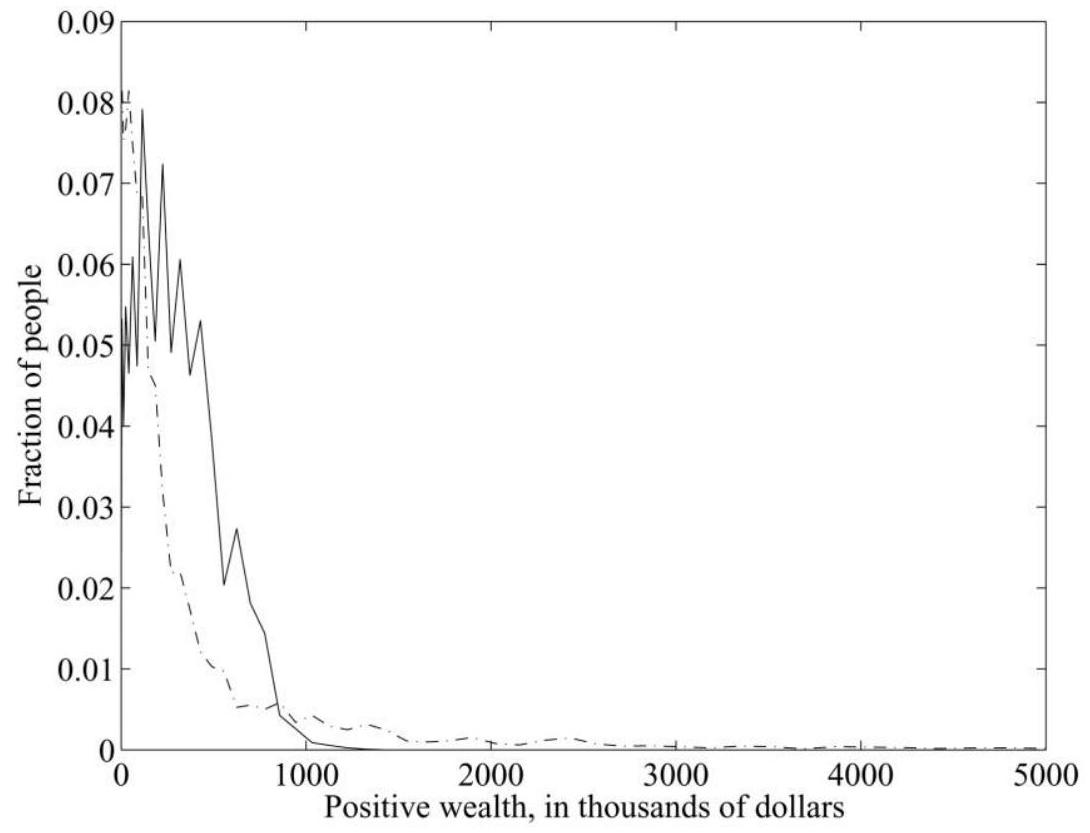
\includegraphics[alt={},max width=\textwidth]{3a7f2112-0917-482b-9d92-bceaeb2d505f-18_833_1090_517_515}
\captionsetup{labelformat=empty}
\caption{Fig. 1.-Distribution of wealth, conditional on wealth being positive, for the whole population. Dash-dot line: data; solid line: model without entrepreneurs.}
\end{center}
\end{figure}

choice. While the data on wealth display a fat tail, in the model without entrepreneurial choice, all households hold less than $\$ 1.1$ million.

\section*{B. The Model with Entrepreneurs}
The third row of table 6 refers to the benchmark economy with entrepreneurs. In our baseline simulation the equilibrium interest rate $r$ is 6.5 percent; the share of total wealth held by entrepreneurs is 29 percent, compared with 33 percent in the data; and the degree of decreasing returns to scale to the entrepreneurial technology is 0.88 , which is a value consistent with those estimated by Burnside, Eichenbaum, and Rebelo (1995) and Basu and Fernald (1997).

This parameterization matches the distribution of wealth very well both for the overall population (fig. 2) and for that of the entrepreneurs (fig. 4).

Figure 3 compares the wealth distributions generated by the model for entrepreneurs and workers. Figure 4 shows the wealth distribution for the subpopulation of entrepreneurs for the model and the data. These pictures reveal two important features of the baseline model. First, and consistent with the data, the distribution of wealth for the popu-

\begin{figure}[h]
\begin{center}
  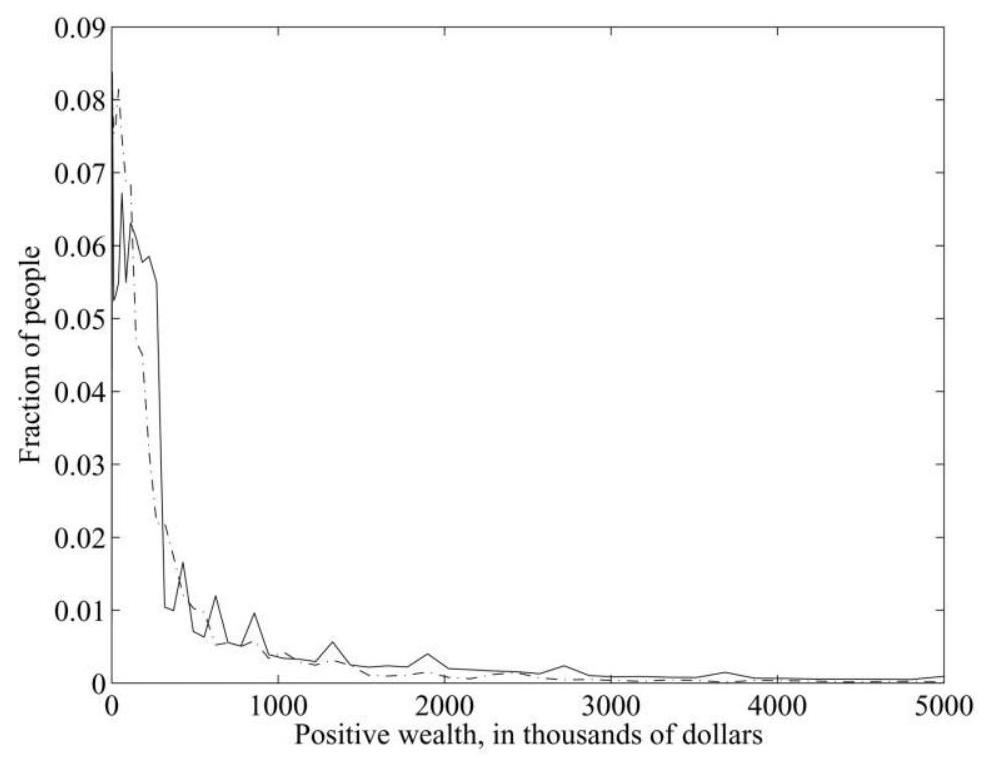
\includegraphics[alt={},max width=\textwidth]{3a7f2112-0917-482b-9d92-bceaeb2d505f-19_761_987_509_567}
\captionsetup{labelformat=empty}
\caption{FIg. 2.-Distribution of wealth, conditional on wealth being positive, for the whole population. Dash-dot line: data; solid line: baseline model with entrepreneurs.}
\end{center}
\end{figure}

\begin{figure}[h]
\begin{center}
  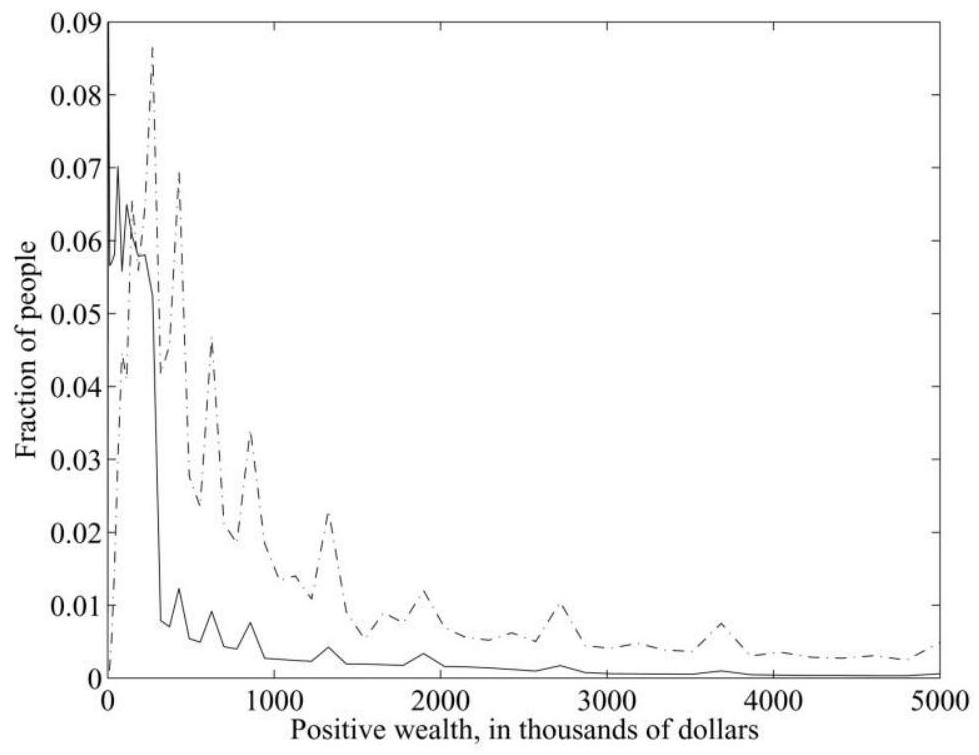
\includegraphics[alt={},max width=\textwidth]{3a7f2112-0917-482b-9d92-bceaeb2d505f-19_755_979_1469_571}
\captionsetup{labelformat=empty}
\caption{FIg. 3.-Distribution of wealth, conditional on wealth being positive, in the baseline model with entrepreneurs. Solid line: workers; dash-dot line: entrepreneurs.}
\end{center}
\end{figure}

\begin{figure}[h]
\begin{center}
  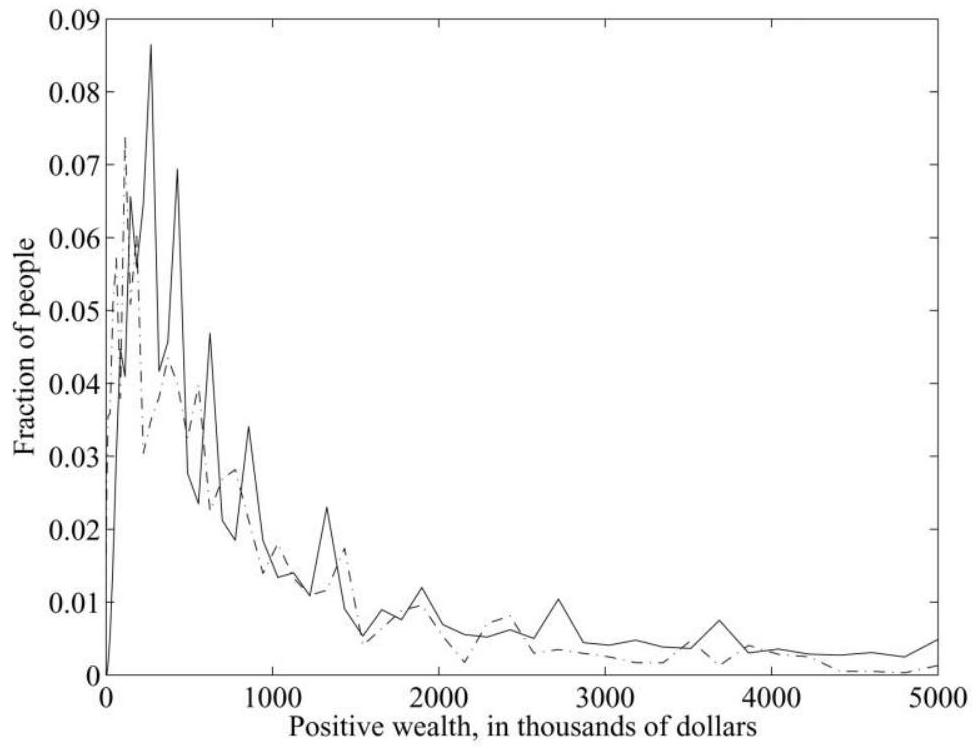
\includegraphics[alt={},max width=\textwidth]{3a7f2112-0917-482b-9d92-bceaeb2d505f-20_749_977_517_573}
\captionsetup{labelformat=empty}
\caption{Fig. 4.-Distribution of the entrepreneurs' wealth, conditional on wealth being positive. Dash-dot line: data; solid line: baseline model.}
\end{center}
\end{figure}

lation of entrepreneurs displays a much fatter tail than the one for workers. Second, contrary to the model without entrepreneurial choice, the baseline model generates distributions of wealth for both entrepreneurs and nonentrepreneurs with a significant mass of people who have more than $\$ 1.1$ million. In the model, the nonentrepreneurs in the right tail of the wealth distribution are former entrepreneurs or descendants of entrepreneurs who have not continued the business of their parents.

In order to explain entrepreneurial behavior, figure 5 displays the saving rate ${ }^{7}$ for people who have the highest ability level as workers during the current period. The solid line refers to the people who get the high entrepreneurial ability level during the current period, and the dash-dot line refers to those who get the low entrepreneurial ability draw. Given the same asset level (and potential earnings as workers), the people with high entrepreneurial ability have a much higher saving rate.

Those with low entrepreneurial ability (who are thus workers) exhibit the buffer stock saving behavior highlighted by Carroll (1997): if their assets are low, they save because they are experiencing a high ability

\footnotetext{${ }^{7}$ The saving rate in the graph is defined as assets in a given period minus assets in the previous period, divided by total income during the period.
}\begin{figure}[h]
\begin{center}
  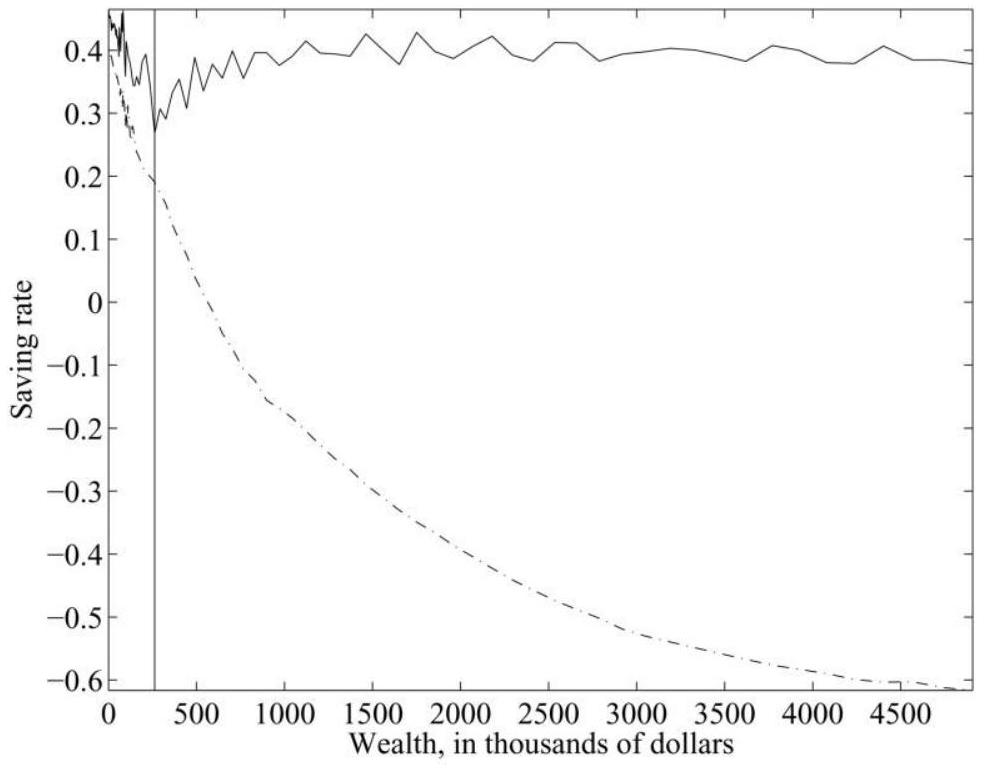
\includegraphics[alt={},max width=\textwidth]{3a7f2112-0917-482b-9d92-bceaeb2d505f-21_768_985_515_569}
\captionsetup{labelformat=empty}
\caption{Fig. 5.-Saving rate for highest-ability workers. Solid line: those with high entrepreneurial ability; dash-dot line: those with no entrepreneurial ability; vertical line: asset level at which high-entrepreneurial ability individuals enter entrepreneurship.}
\end{center}
\end{figure}

level as workers and want to build up their buffer stock. If their assets are high enough, they dissave; and the richer they are, the higher their rate of dissaving. In this simulation, the asset level at which the saving rate goes from positive to negative is below $\$ 1$ million.

The people with high entrepreneurial ability become entrepreneurs only if their wealth is above a certain level, denoted in the graph by a vertical line. The saving rate of those with high entrepreneurial ability who do not own enough assets to become entrepreneurs is higher than the one for the workers because ability is persistent, and the workers with high entrepreneurial ability save to have a chance to start a business in the future. In this region, the distance between the solid line and the dash-dot line is solely due to the higher implicit rate of return from saving that one could obtain becoming an entrepreneur in the future: all households become workers in this range and earn the same income, but the desire to become entrepreneurs generates a higher saving rate for those who have such ability.

The saving rate of those with high entrepreneurial ability and enough assets to become entrepreneurs is positive and considerably higher than that for workers. The return on the entrepreneurial activity is high, and the entrepreneur would like to increase the size of the firm by borrowing

\begin{figure}[h]
\begin{center}
  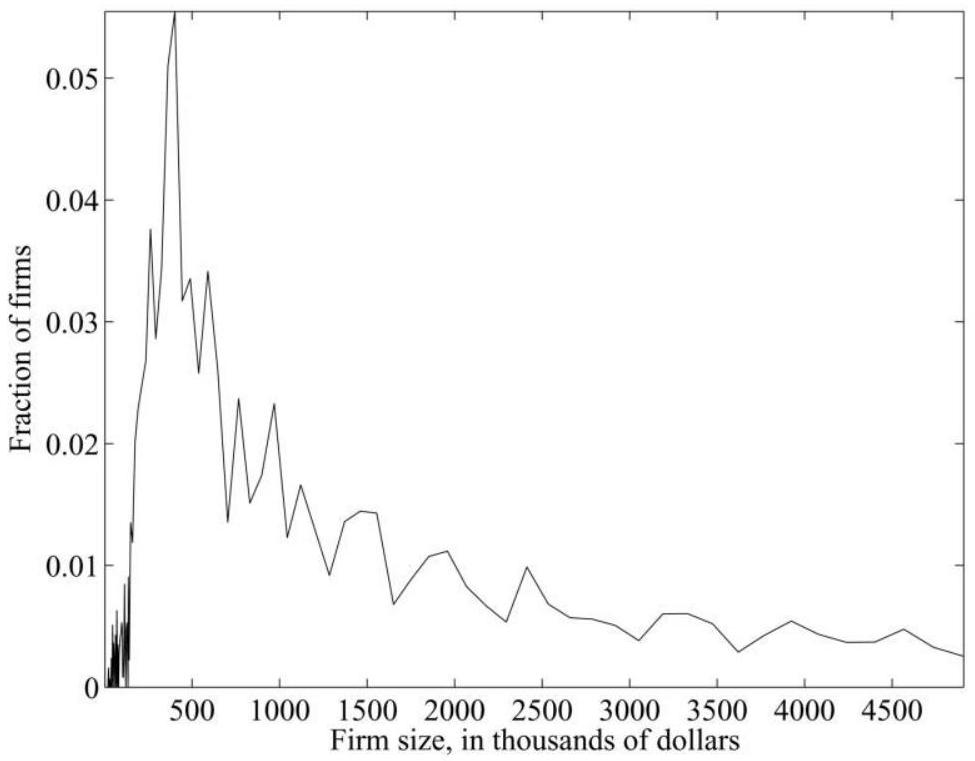
\includegraphics[alt={},max width=\textwidth]{3a7f2112-0917-482b-9d92-bceaeb2d505f-22_761_975_509_577}
\captionsetup{labelformat=empty}
\caption{Fig. 6.-Firm size distribution, baseline model with entrepreneurs}
\end{center}
\end{figure}

capital. However, the borrowing constraint limits the size of the firm. In order to expand the business, the entrepreneur must in part selffinance the increase in capital. The combination of higher returns from the business together with the budget constraint thus generates a very high saving rate for entrepreneurs. As the firm expands, the returns decrease. Therefore, the saving rate will also eventually decrease. (We truncate the axis of the graph for easier readability.)

With only one positive level of entrepreneurial ability (as we assume in our calibration) and in the absence of borrowing constraints, there would be only one optimal firm size. Figure 6 shows how in our framework borrowing constraints can generate a large amount of heterogeneity in the firm size distribution. The distribution generated by the model exhibits high dispersion and a fat tail; the tail is generated by the entrepreneurs who have remained in business for a long period (and have possibly inherited the firm from their parents) and have thus had time to save and increase the size of their firms.

\section*{C. The Borrowing Constraints}
In this subsection, we examine the effect of changing the tightness of the borrowing constraints. To make the constraints more stringent, we increase $f$, the fraction of working capital that cannot be seized by cred-

\begin{figure}[h]
\begin{center}
  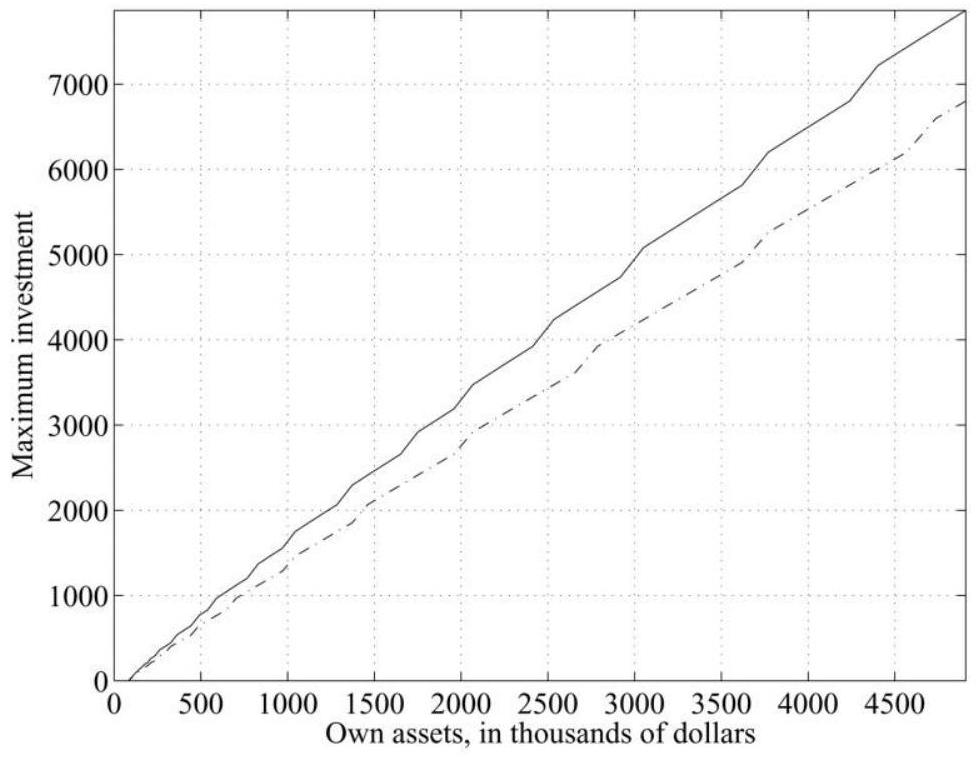
\includegraphics[alt={},max width=\textwidth]{3a7f2112-0917-482b-9d92-bceaeb2d505f-23_757_979_509_575}
\captionsetup{labelformat=empty}
\caption{Fig. 7.-Maximum investment. Solid line: baseline; dash-dot line: more restrictive borrowing constraints.}
\end{center}
\end{figure}

itors, from 0.75 to 0.85 . The more the entrepreneur can appropriate in case of default, the stronger the incentive to default for a given collateral level, and the less the creditor is willing to lend. This increase in $f$ could be interpreted as less efficient enforcement of property rights by the courts, or as more lenient bankruptcy laws.

Figure 7 shows the maximum amount of investment (including one's own assets and borrowed funds) for a young entrepreneur who has the highest ability level as a worker as a function of his own assets. The solid line refers to the baseline model, and the dash-dot line refers to the model with more restrictive borrowing constraints (and nonrecalibrated $\beta)$. In both economies the entrepreneurs with few assets cannot borrow. The amount of collateral necessary to borrow a positive amount in the two economies coincides at low levels of assets. The entrepreneur with the lowest ability level as a worker must have at least $\$ 10,000$ in order to borrow some funds; this amount increases to $\$ 86,000$ for the entrepreneur with the highest ability level as a worker. This happens because a more able worker is better off in case of default; therefore, he has to provide more collateral. The key difference in the two economies is that richer entrepreneurs can borrow and invest less in the economy with more restrictive borrowing constraints. For this reason they need more initial assets to implement a project of a given size, and it takes\\
them longer to become rich and own and run a large firm. If the entrepreneur is rich enough, he is unconstrained.

The first two lines of table 7 report, respectively, selected statistics of the U.S. data and of the baseline calibration. The third line of table 7 reports the effects of more restrictive borrowing constraints. The capitaloutput ratio drops drastically, from 3.0 to 2.7 , and the fraction of entrepreneurs falls from 7.5 percent to 6.9 percent since fewer high-ability individuals can now borrow and start a firm. The decrease in the fraction of entrepreneurs happens despite an increase of the equilibrium interest rate from 6.5 percent to 7.5 percent, which makes it easier (and faster) for savers with high entrepreneurial ability to accumulate enough capital to start a business.

An increase in the tightness of the borrowing constraint, as seen in figure 7, forces entrepreneurs, and in particular rich ones, to borrow less and to run smaller firms. They make fewer total profits and save less, and as a result, they are poorer. The distribution of wealth becomes less concentrated; for instance, the share of total net worth held by the richest 1 percent decreases from 31 percent in the baseline calibration to 24 percent, and the share of total net worth held by entrepreneurs decreases from 29 percent to 25 percent. Hence, as the collateral requirements rise, wealth inequality falls, but this comes at the expense of lower capital accumulation and output.

\section*{D. Bequests}
In the baseline economy households are altruistic toward their offspring; therefore, the total amount of bequests includes both voluntary and accidental bequests due to life span risk. We use our model to study what happens to entrepreneurial choice and to wealth inequality when households do not care about their descendants and all bequests are accidental.

The fourth line of table 7 displays how the aggregates change when we set to zero the degree of intergenerational altruism. The absence of the voluntary bequest motive reduces the incentives to accumulate capital and run larger and larger firms. On the one hand, younger people are bequeathed less wealth, and in the presence of borrowing constraints, this means that young potential entrepreneurs have fewer resources to start and increase their businesses. On the other hand, the equilibrium interest rate increases to 9.3 percent, thus allowing more high-ability individuals to use the increased proceeds from their earnings to start a business activity. As a result, the fraction of entrepreneurs is roughly unchanged.

The effects on aggregate capital accumulation are large: in the absence of a voluntary bequest motive to save, the total capital of the

\begin{table}[h]
\begin{center}
\captionsetup{labelformat=empty}
\caption{TABLE 7\\
The Role of Borrowing Constraints and Voluntary Bequests}
\begin{tabular}{|l|l|l|l|l|l|l|l|l|}
\hline
\multirow{2}{*}{} & \multirow[b]{2}{*}{CapitalOutput Ratio} & \multirow[b]{2}{*}{Interest Rate} & \multirow[b]{2}{*}{Wealth Gini} & \multirow[b]{2}{*}{Entrepreneurs} & \multicolumn{4}{|c|}{Percentage Wealth in the Top} \\
\hline
 &  &  &  &  & 1\% & 5\% & 20\% & 40\% \\
\hline
U.S. data & 3.0 & . . . & . 8 & 7.55\% & 30 & 54 & 81 & 94 \\
\hline
Baseline with entrepreneurs & 3.0 & 6.5\% & . 8 & 7.50\% & 31 & 60 & 83 & 94 \\
\hline
More stringent borrowing constraints: $f=.85$ & 2.7 & 7.5\% & . 7 & 6.90\% & 24 & 49 & 75 & 91 \\
\hline
No altruism: $\eta=0$, only involuntary bequests & 2.5 & 9.3\% & . 7 & 7.55\% & 21 & 45 & 73 & 90 \\
\hline
$\eta=0$, recalibrated $\beta=.88$ & 3.0 & 6.4\% & . 8 & 7.9\% & 28 & 57 & 81 & 94 \\
\hline
\end{tabular}
\end{center}
\end{table}

economy would decrease from 3.0 to 2.5. The concentration of wealth would also drop substantially: the Gini coefficient of inequality would go from 0.8 to 0.7 , and the fraction of wealth held by the richest 1 percent from 31 percent to 21 percent. As also shown by De Nardi (2004), voluntary bequests are fundamental in explaining the concentration of wealth.

In this model economy, voluntary bequests provide rich entrepreneurs with an additional incentive to save and also generate the intergenerational transmission of large fortunes (and firms) across generations.

To better understand the role of voluntary bequests, we run another experiment (last line of the table) in which we increase the discount factor $\beta$ to .882 (up from .867 in the baseline calibration) to match a capital-output ratio of 3.0. The fraction of entrepreneurs increases compared to the baseline model, from 7.5 percent to 7.9 percent. This effect is mainly due to the increase in the household's discount factor $(\beta)$. In this calibration, households have no bequest motive but are more patient. This implies that the younger households accumulate more wealth than in the baseline model, whereas the old decumulate faster, and thus keep less wealth, because of the lack of altruism. More people of working age become entrepreneurs, and the old have fewer incentives to continue and expand the entrepreneurial activity and pass to their offspring less wealth and smaller firms. This reduces the number and the size of large firms. For these reasons, the wealth concentration generated by this experiment is lower than the one in the benchmark economy and in the actual data; for instance, the share of total net worth held by the richest 1 percent drops to 28 percent, down from 31 percent in the baseline economy.

\section*{V. Inspecting the Model's Mechanisms}
Recent literature has cast doubt on the relevance of borrowing constraints to entrepreneurial entry (Hurst and Lusardi 2004) and on the size of the returns to entrepreneurship (Moskowitz and VissingJørgensen 2002). High wealth inequality in our model is generated by the combination of occupational choice in the presence of borrowing constraints and high potential returns to entrepreneurship. We check here whether the observable implications generated by our model are consistent with the observed data that are the focus of these two papers.

\section*{A. Borrowing Constraints}
The main finding of Hurst and Lusardi (2004) is that the probability of entering entrepreneurship is almost flat over a large portion of the wealth distribution and then increases for the richest workers. On the\\
basis of this finding one might (erroneously) conclude that entrepreneurs are not borrowing constrained.

There are two main points worth discussing. The first point is that the results of our paper do not depend in important ways on the fact that the financial constraint affects the decision to become an entrepreneur. Rather, it is the greater incentive to save after entry that is crucial for the results. We have run and calibrated versions of the model in which people retain labor income upon entering entrepreneurship and in which, therefore, the entry decision does not depend on wealth, but only on entrepreneurial ability. This version of the model produces numbers that are quantitatively very close to those in the other version, and all the conclusions that we draw in the paper remain the same.

The second point is that our model of occupational choice with borrowing constraints produces entry decisions that are consistent with Hurst and Lusardi's finding. To check on this we proceed as follows. We generate many samples of households from our model, each of which is of the same size as those of Hurst and Lusardi's sample. We then use each sample to estimate a probit regression, according to which the probability of entering entrepreneurship is a function of a fifthorder polynomial in the household's own wealth, controlling for income, age, and previous entrepreneurial status. ${ }^{8}$ We finally use the estimated probit coefficients from all these samples to construct 95 percent confidence intervals for the estimated probability of entry as a function of wealth (we fix all other controls at their mean).

Figures $8 a$ and $b$ plot Hurst and Lusardi's estimated function (dashed line) and the confidence intervals (between the two solid lines) generated by two versions of our model. Figure $8 a$ refers to our benchmark model. Two features are worth noticing: first, the entry probabilities implied by the benchmark model are lower than in Hurst and Lusardi's sample. This makes sense since the relevant notion of entrepreneurship for our model ( 7.5 percent of households are entrepreneurial households) is more restricted than the one in their sample (they do not report the exact number, but our calculations with the PSID bound it between 11 percent and 13 percent). If the relevant fraction of "entrepreneurs" in the population is higher, so is the entry probability.

Second, both Hurst and Lusardi's estimates and our confidence intervals are consistent with an entry probability that is a convex function of wealth. The intuition is linked to the endogeneity of both wealth and entry into entrepreneurship. In the presence of borrowing constraints, a worker with high entrepreneurial ability is likely to save to enter entrepreneurship. As a result, when observing a cross section of people,

\footnotetext{${ }^{8}$ We do not need to condition on education, gender, marital status, and race, since such dimensions of heterogeneity are absent from our model.
}\begin{figure}[h]
\begin{center}
  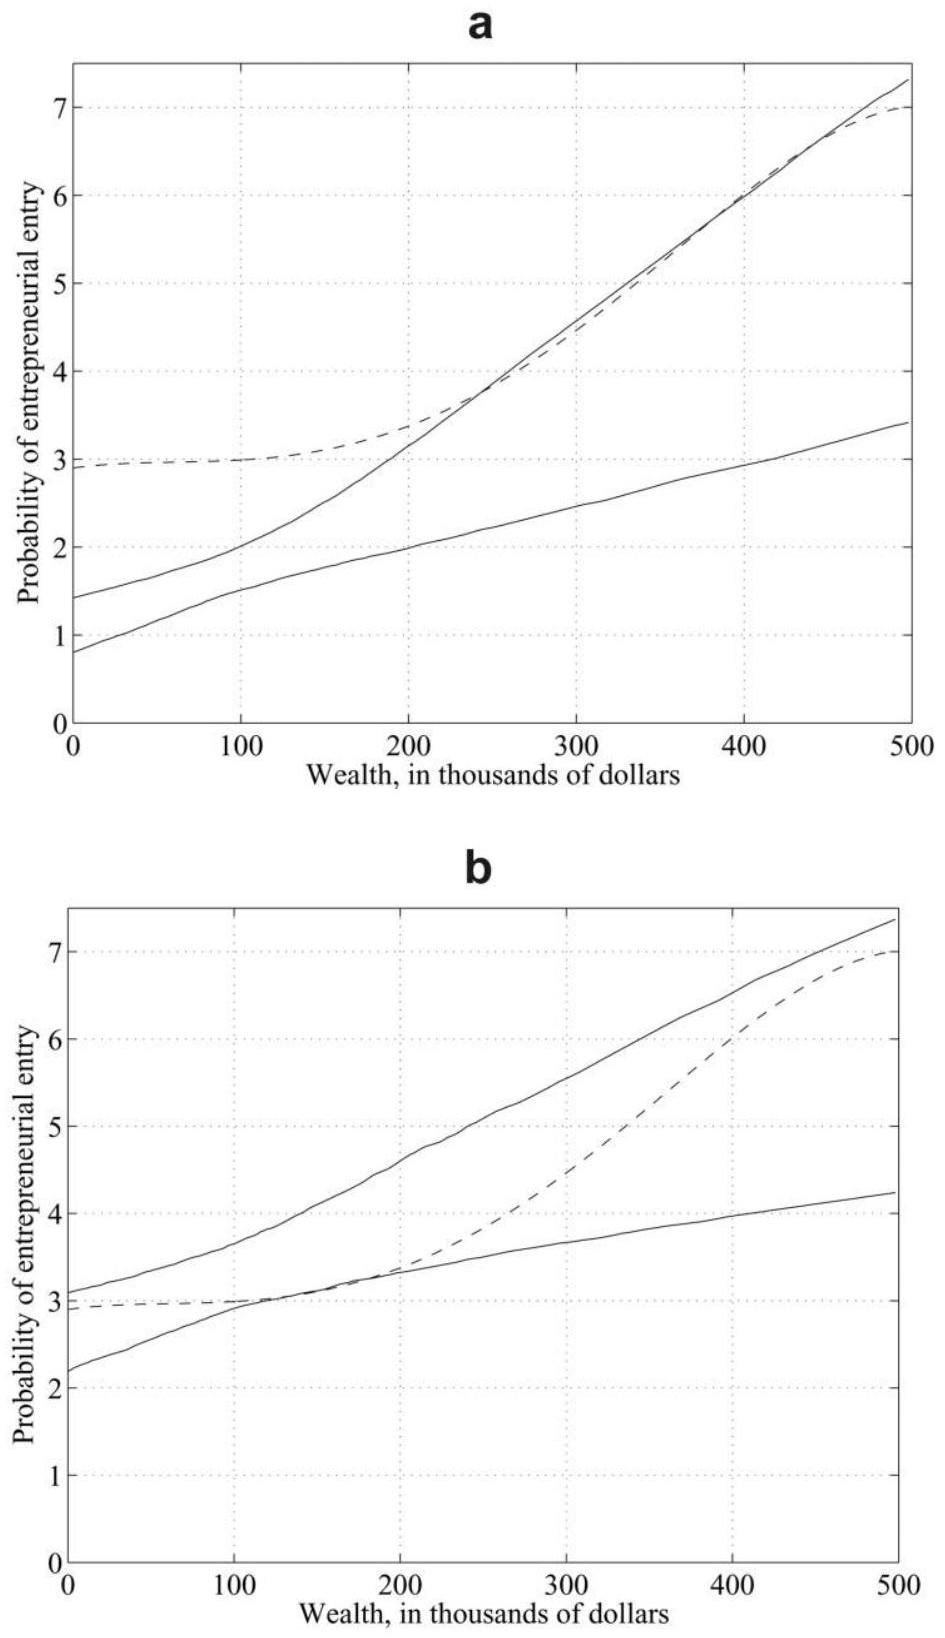
\includegraphics[alt={},max width=\textwidth]{3a7f2112-0917-482b-9d92-bceaeb2d505f-28_1638_945_526_592}
\captionsetup{labelformat=empty}
\caption{Fig. 8.-Probability of entering entrepreneurship as a function of own wealth as estimated by Hurst and Lusardi (dashed line), and confidence interval generated by two versions of the model (solid lines). $a$, Benchmark model. $b$, Benchmark with a small fraction of nonentrepreneurial self-employed.}
\end{center}
\end{figure}

we are not very likely to observe many high-ability potential entrepreneurs among the poor. On the other hand, several of the rich workers are those workers who have high ability as entrepreneurs and have been saving to accumulate enough wealth to enter entrepreneurship. For this reason, if we give an extra dollar to someone in the lower part of the distribution, this person is not very likely to enter entrepreneurship; whereas if we give a dollar to someone who is wealthier, he is more likely to be around the entry threshold and thus to enter entrepreneurship. Our estimates for this definition of entrepreneurship, however, predict a steeper positive relationship at low levels of wealth than the one estimated by Hurst and Lusardi.

As we discussed, there is a lot of heterogeneity among the households that report being self-employed or business owners, and those that are called entrepreneurs in the data (and in Hurst and Lusardi's paper as well) are not necessarily all entrepreneurs in the sense of our model. Figure $8 b$ estimates the same regression in the case in which a subset of the simulated agents who are workers for the purposes of our model ${ }^{9}$ are classified as self-employed workers and counted as entrepreneurs for the purpose of comparing our results with the survey data. ${ }^{10}$ While stylized, this experiment is very instructive: the function estimated by Hurst and Lusardi now falls within our 95 percent model-generated confidence interval. Given that we assume only one type of entrepreneurial ability and that none of the calibrated parameters were chosen to match this aspect of the data, it is remarkable how our model is not inconsistent with flat entry probabilities over large sections of wealth holdings.

Consistent with our findings, Buera (2006) estimates a model of entrepreneurial choice and finds that allowing for a slightly more general formulation of entrepreneurial heterogeneity can do an even better job of matching the estimated entry probability.

\section*{B. Returns from Private Business Ownership}
Moskowitz and Vissing-Jørgensen's (2002) computations cast doubt on the assumption that entrepreneurs face potentially high rates of return.

\footnotetext{${ }^{9}$ Notice that being an "entrepreneur" in our model is a statement about the household's production function and rate of return from saving. It is not a statement on who the household's employer is, where they work, the flexibility of hours worked, and so on.\\
${ }^{10}$ We choose this fraction so that the entrepreneurs (including the true ones in the sense of our model) in our model-generated data are about 12 percent of the sample (a number similar to the one in Hurst and Lusardi's sample). We assume that all workers across the wealth distribution have a constant probability of becoming nonentrepreneurial self-employed and that this probability is uncorrelated with all other characteristics. We also assume that the probability of exiting the nonentrepreneurial self-employed status is the same as exiting entrepreneurship, but the results are not very sensitive to this assumption.
}\begin{table}[h]
\begin{center}
\captionsetup{labelformat=empty}
\caption{TABLE 8\\
Distribution of Rates of Return (\%) for Self-Employed Business Owners}
\begin{tabular}{lcccc}
\hline\hline
 & \multicolumn{4}{c}{Percentile} \\
\cline { 2 - 5 }
 & 25 th & 50 th & 75 th & 90 th \\
\hline
Only income from business & 0 & 3 & 25 & 143 \\
Including wages and salaries & 10 & 40 & 125 & 520 \\
\hline
\end{tabular}
\end{center}
\end{table}

Note.-Returns are entrepreneurial income divided by business net worth. In the first line, entrepreneurial income includes only income or loss from business. The second line also includes wages and salaries received by the business owner.

Their computations are complex because their goal is to compare aggregate returns to private and public equity, and they thus need to adjust their computations for firms' entry and exit.

Given that our goal is to compare returns to entrepreneurship in the data and in our model and that our framework explicitly deals with entrepreneurial mobility, we compare the cross-sectional distribution of returns to entrepreneurship in a given period in our model and in the data. Consistent with our model, we compute this distribution of returns for the self-employed business owners (who are a subset of all those who hold private equity) using the 1989 SCF wave (table 8). These returns are computed as entrepreneurial income divided by business net worth.

Interestingly, we find that the size of the returns to private equity crucially hinges on how income from the firm is divided between entrepreneurial wages and return to capital. It is well known that this split is in practice arbitrary and likely to depend on tax incentives and possibly other considerations. In the SCF data, if one does not include the selfreported wages and salaries, such a rate of return is 3 percent for the entrepreneurs in the fiftieth percentile and 143 percent for those in the top 10 percent. If, as an extreme case, all wages and salaries received by the entrepreneurs are included in the computation of such returns, the corresponding numbers become 40 percent and 520 percent, which are far bigger numbers.

In our model, it is not clear how one should compute wages for the entrepreneurs. One could take the view that their labor income is the shadow one, meaning the one that they could make if they were to work as workers (which is not observed in the SCF data). But one could equally plausibly assume that entrepreneurial profits should be computed as the amount of entrepreneurial capital times the rate of return from capital in our economy (which is 6.5 percent), and the rest of the entrepreneurial income is due to entrepreneurial talent and should thus be attributed to entrepreneurial wages. Given the arbitrariness of this split, we believe that the returns to be compared in our model and the data should be computed by using total income from the entrepreneurial business activity, both in our model and in the data.

Given that our model, by design, abstracts from many aspects of entrepreneurial choice, the distribution of returns is less disperse in our model than in the data. We thus compare the median distribution of returns, which is 49 percent in our model compared to 40 percent in the data. Our median entrepreneurial return is thus only a little higher in our model than in the SCF data.

There are two reasons why our computed return is overstated compared to the one computed in the SCF data. First, households tend to underreport income. Research by the Internal Revenue Service (IRS) (Plate et al. 1990) computes business income underreporting for the 1985-92 period ranging from 28 percent to 40 percent. The SCF data are not collected for tax purposes, and it is possible that the households underreport less to the SCF than to the IRS. To be conservative, we compute the implied median return in our economy for $10-20$ percent business income underreporting. The corresponding median returns become 43 percent and 36 percent, respectively. Second, the computed return from our model does include capital gains (which, for the purpose of our model, are indistinguishable from other entrepreneurial income), whereas, because of available data limitations, the returns computed from the SCF do not include capital gains. We thus conclude that entrepreneurial returns in our model are consistent with those measured in the data.

\section*{VI. Conclusions}
We developed and solved numerically a model of occupational choice, wealth accumulation, and bequests in which entrepreneurs face an endogenous borrowing constraint that limits the amount that they can borrow. The entrepreneur's wealth acts as collateral, so the richer the entrepreneur, the higher the amount that he can borrow.

A very parsimonious parameterization of our model generates a wealth distribution that matches the one observed in the data, both for entrepreneurs and for workers. It also produces returns from entrepreneurship and households' entry probabilities into entrepreneurship as a function of one's wealth, which are consistent with the ones measured in the data. None of the parameters of the model were chosen to obtain these results.

The key mechanism is that many entrepreneurs face potentially high rates of return but are constrained in the amount that they can borrow. To expand their firm, these entrepreneurs keep saving. In doing so, they become richer and richer. The most successful dynasties share their fortunes with their children, some of whom will keep the family firm going, thus expanding the dynasty's fortune even more.

We show that the tightness of borrowing constraints and voluntary\\
bequests are main forces in determining the number of entrepreneurs, the size of their firms, the overall wealth concentration in the population, and the aggregate capital accumulation.

These results have implications for policy analysis, such as subsidized loans to entrepreneurs and estate taxes. Subsidized loans would make it cheaper for the entrepreneurs to borrow but would also change their incentives to default, making the effects of this policy a priori ambiguous. Taxing bequests may decrease inequality, while at the same time reducing the amount of entrepreneurial wealth that could be used as collateral, and thus may affect both the number of entrepreneurs and the total capital of the economy, as shown by Cagetti and De Nardi (2004).

We have assumed that an agent can exploit one's own entrepreneurial ability only by starting and developing a business. In the presence of borrowing constraints the entrepreneur might want to sell his idea or project to another, potentially less constrained, party. In many situations, however, markets for ideas or projects are very limited. Potential explanations for this, first expressed in Arrow's work (1962), are that informational problems may prevent potential buyers from evaluating the entrepreneur's project and also that the innovating entrepreneur may have problems in appropriating the returns from his idea because it might be too complex to write or enforce a contract specifying the usage of the idea and the payments for information. In our model there are two sectors: entrepreneurial and nonentrepreneurial firms. Only part of the productive and inventive activity is generated by the constrained sector; the rest is generated by nonentrepreneurial firms, which face no borrowing constraints, and in which it does not matter who develops the idea and who implements it. We leave all these issues for future research.

\section*{Appendix A}
\section*{Income and Entrepreneurial Ability Processes}
We assume that the income process is lognormal and $\mathrm{AR}(1)$. We approximate it with a five-point discrete Markov chain, using the method described in Tauchen and Hussey (1991).

The resulting grid points for the vector $\boldsymbol{y}$ for the income process (normalized to an average of one) are

$$
\left[\begin{array}{lllll}
.2468 & .4473 & .7654 & 1.3097 & 2.3742],
\end{array}\right.
$$

and the transition matrix $\mathbf{P}_{y}$ is

$$
\begin{array}{lllll}
.7376 & .2473 & .0150 & .0002 & .0000 \\
.1947 & .5555 & .2328 & .0169 & .0001 \\
.0113 & .2221 & .5333 & .2221 & .0113 \\
.0001 & .0169 & .2328 & .5555 & .1947 \\
.0000 & .0002 & .0150 & .2473 & .7376
\end{array}
$$

We assume that the entrepreneurial ability process is uncorrelated with the income process. The two values for ability $\boldsymbol{\theta}$ are zero (meaning no entrepreneurial ability) and a positive value (0.514), and the transition matrix $\mathbf{P}_{\theta}$ is

$$
\left[\begin{array}{ll}
.964 & .036 \\
.206 & .794
\end{array}\right]
$$

\section*{Correlation between Abilities}
We have so far assumed that working ability ( $y$ ) and entrepreneurial ability ( $\theta$ ) are uncorrelated. It is difficult to measure such correlation in the data. While many entrepreneurs are high-ability individuals who would have high earnings if employed by a company, other successful entrepreneurs may do poorly if they were to work for a corporation.

One important piece of evidence in favor of our specification is that we replicate fairly well the income of entrepreneurs prior to starting their businesses. Using the PSID, one can compare household previous labor incomes for individuals who subsequently decide to either enter entrepreneurship or remain workers in a given period. Hurst and Lusardi (2004) report that the labor earnings over the previous five years of those who enter entrepreneurship in a given period are 1.32 times the labor income during the previous five years of those who choose to remain workers in the same period. Our simulations reproduce this feature: the ratio of the incomes for the two groups (entrants and nonentrants) is 1.35 . This correlation arises endogenously in our model. Because of borrowing constraints, high-entrepreneurial ability workers save to reach their constrained optimal firm size at entry. Among the high-entrepreneurial ability workers, those who receive high labor earnings realizations can save more and are thus more likely to accumulate enough capital and to enter entrepreneurship.

Moreover, as a robustness check, we also study the effects of allowing for positive correlation between these two ability processes. To make this comparison as clean as possible, we keep the marginal distributions and transition probabilities as in the baseline case. We then assume that the two processes have a positive correlation of 0.4 . All other parameters are as in the baseline economy, except for the discount factor $\beta$, which we recalibrate to obtain the same capitalincome ratio as in the benchmark. In this economy, the ratio of labor income over the previous five periods for entrants and nonentrants becomes 1.59 , which is higher than the one observed in the data. The resulting wealth distribution is close to the one in our benchmark economy: the richest 1 percent hold 33 percent of the total wealth, and the richest 5 percent hold 63 percent. The main difference is that in this economy the number of entrepreneurs decreases to 5.2 percent. This happens because in the presence of positive correlation between the two dimensions of abilities, people with high entrepreneurial ability tend to have a higher option value of remaining in the nonentrepreneurial\\
sector and are thus less likely to become entrepreneurs. It is worth noting that this feature does not significantly affect the right tail of the wealth distribution and the saving and investment behavior of the richest entrepreneurs. As we have already mentioned, this tail is composed of the few entrepreneurs who have remained successful for several periods and who have therefore managed to increase their business.

\section*{Appendix B}
\section*{The Algorithm}
The algorithm proceeds as follows.

\begin{itemize}
  \item Construct a grid for the state variables. The maximum asset level is chosen so that it is not binding for the household's saving decisions.
  \item Fix a tax rate $\tau$, an interest rate $r$, and a wage rate $w$. Taking these as given, solve for the value functions using a value function iteration.
  \item Construct the transition matrix M. Compute the associated invariant distribution over states, starting from a guess for $\boldsymbol{\pi}$ and iterating on $\boldsymbol{\pi}^{\prime}= \mathbf{M} \boldsymbol{\pi}$ until $\boldsymbol{\pi}^{\prime}-\boldsymbol{\pi}$ is smaller than a given convergence criterion.
  \item Compute total savings and total capital invested in the entrepreneurial sector implied by the invariant distribution. Total capital invested by the nonentrepreneurial sector is given by the difference between total savings and total capital invested by the entrepreneurs.
  \item Compute $r$ and $w$ implied by the above quantities and the nonentrepreneurial aggregate production function, update the wage and interest rate used to solve the problem, and iterate until convergence on the factor prices is reached.
  \item Compute the social security system imbalance and iterate on $\tau$ until outlays equal revenues.
\end{itemize}

The computation of the value functions is nonstandard because of the endogenous borrowing constraints. For each state $\boldsymbol{x}$, the endogenous borrowing constraint specifies a maximum amount $k(\boldsymbol{x})$ that an entrepreneur can borrow. The specific function $k$ depends, however, on the value functions themselves. In the algorithm we exploit the fact that, for a given set of state variables, if an entrepreneur runs away with a given level of capital $k$, he would also run away with any $k+\epsilon$, where $\epsilon \geq 0$. We adopt the following algorithm: initialize $\hat{k}(\boldsymbol{x})=k_{\text {max }}$, the maximum investment level in the economy. We solve the value functions, iterating until convergence, conditional on this borrowing constraint. For each value of $\boldsymbol{x}$, we compare the value function associated with remaining an entrepreneur and repaying the debt with the value function associated with default; we find the maximum level of investment (and borrowing) for which the entrepreneur would not default and set the new $\hat{k}(\boldsymbol{x})$ to this new value, and compute again the value functions conditional on this updated constraint. This procedure is iterated until $\hat{k}$ does not change across iterations.

Because we do not constrain the $\hat{k}(\boldsymbol{x})$ functions to be decreasing when we iterate on them, we are not imposing convergence. Together with the initialization of these functions at the maximum possible level of borrowing, this implies that if the model has more than one solution and if the algorithm converges monotonically, then we converge to the "best" solution, that is, the one that allows for the most borrowing in the economy. In all our simulations the algorithm did converge monotonically.

\section*{References}
Albuquerque, Rui, and Hugo A. Hopenhayn. 2004. "Optimal Lending Contracts with Imperfect Enforceability." Rev. Econ. Studies 71 (April): 285-315.\\
Arrow, Kenneth J. 1962. "Economic Welfare and the Allocation of Resources for Invention." In The Rate and Direction of Inventive Activity: Economic and Social Factors. Princeton, NJ: Princeton Univ. Press (for NBER).\\
Attanasio, Orazio P., James Banks, Costas Meghir, and Guglielmo Weber. 1999. "Humps and Bumps in Lifetime Consumption." J. Bus. and Econ. Statis. 17 (January): 22-35.\\
Auerbach, Alan J., and Laurence J. Kotlikoff. 1995. Macroeconomics: An Integrated Approach. Cincinnati: South-Western.\\
Basu, Susanto, and John G. Fernald. 1997. "Returns to Scale in U.S. Production: Estimates and Implications." J.P.E. 105 (April): 249-83.\\
Berkowitz, Jeremy, and Michelle J. White. 2004. "Bankruptcy and Small Firms' Access to Credit." Rand J. Econ. 35 (Spring): 69-84.\\
Bewley, Truman F. 1977. "The Permanent Income Hypothesis: A Theoretical Formulation." J. Econ. Theory 16 (December): 252-92.\\
Blanchard, Olivier J. 1985. "Debt, Deficits, and Finite Horizons." J.P.E. 93 (April): 223-47.\\
Buera, Francisco. 2006. "Persistency of Poverty, Financial Frictions, and Entrepreneurship." Manuscript, Northwestern Univ., Dept. Econ.\\
Burnside, Craig, Martin Eichenbaum, and Sergio Rebelo. 1995. "Capital Utilization and Returns to Scale." In NBER Macroeconomics Annual 1995, edited by Ben S. Bernanke and Julio J. Rotemberg. Cambridge, MA: MIT Press.\\
Cagetti, Marco, and Mariacristina De Nardi. 2004. "Taxation, Entrepreneurship and Wealth." Staff Report no. 340, Fed. Reserve Bank Minneapolis.\\
-. 2005. "Wealth Inequality: Data and Models." Working Paper no. 200510, Fed. Reserve Bank Chicago.\\
Carroll, Christopher D. 1997. "Buffer Stock Saving and the Life Cycle/Permanent Income Hypothesis." Q.J.E. 112 (February): 1-55.\\
Castañeda, Ana, Javier Díaz-Giménez, and José-Víctor Ríos-Rull. 2003. "Accounting for the U.S. Earnings and Wealth Inequality." J.P.E. 111 (August): 81857.

Cooley, Thomas, Ramon Marimon, and Vincenzo Quadrini. 2004. "Aggregate Consequences of Limited Contract Enforceability." J.P.E. 112 (August): 81747.

Curtin, Richard T., F. Thomas Juster, and James N. Morgan. 1989. "Survey Estimates of Wealth: An Assessment of Quality." In The Measurement of Saving, Investment and Wealth, edited by Robert E. Lipsey and Helen Stone Tice. Chicago: Univ. Chicago Press (for NBER).\\
De Nardi, Mariacristina. 2004. "Wealth Inequality and Intergenerational Links." Rev. Econ. Studies 71 (July): 743-68.\\
Eisfeldt, Andrea L., and Adriano A. Rampini. 2005. "New or Used? Investment with Credit Constraints." Manuscript, Northwestern Univ., Kellogg School Management.\\
Evans, David S., and Boyan Jovanovic. 1989. "An Estimated Model of Entrepreneurial Choice under Liquidity Constraints." J.P.E. 97 (August): 808-27.\\
Gentry, William M., and R. Glenn Hubbard. 2004. "Entrepreneurship and Household Savings." Advances Econ. Analysis and Policy 4 (1): art. 8. \href{http://www}{http://www} .bepress.com/bejeap/advances/.\\
Gertler, Mark. 1999. "Government Debt and Social Security in a Life-Cycle Economy." Carnegie-Rochester Conf. Ser. Public Policy 50 (June): 61-110.

Gollin, Douglas. 2002. "Getting Income Shares Right." J.P.E. 110 (April): 45874.

Holtz-Eakin, Douglas, David Joulfaian, and Harvey S. Rosen. 1994. "Sticking It Out: Entrepreneurial Survival and Liquidity Constraints." J.P.E. 102 (February): 53-75.\\
Hurst, Erik, and Annamaria Lusardi. 2004. "Liquidity Constraints, Household Wealth, and Entrepreneurship." J.P.E. 112 (April): 319-47.\\
Kehoe, Timothy J., and David K. Levine. 1993. "Debt-Constrained Asset Markets." Rev. Econ. Studies 60 (October): 865-88.\\
Kotlikoff, Laurence J., Kent A. Smetters, and Jan Walliser. 1999. "Privatizing Social Security in the United States-Comparing the Options." Rev. Econ. Dynamics 2 (July): 532-74.\\
Lucas, Robert E., Jr. 1978. "On the Size Distribution of Business Firms." Bell J. Econ. 9 (Autumn): 508-23.\\
Marcet, Albert, and Ramon Marimon. 1992. "Communication, Commitment, and Growth." J. Econ. Theory 58 (December): 219-49.\\
Moskowitz, Tobias J., and Annette Vissing-Jørgensen. 2002. "The Returns to Entrepreneurial Investment: A Private Equity Premium Puzzle?" A.E.R. 92 (September): 745-78.\\
Plate, Roger L., Gary P. Bingham, Dennis R. Cox, Berdj Kenadjian, and Alan H. Plumley. 1990. "Income Tax Compliance Research: Net Tax Gap and Remittance Gap Estimates." Supplement to Publication 7285, Internal Revenue Service, Washington, DC.\\
Quadrini, Vincenzo. 1999. "The Importance of Entrepreneurship for Wealth Concentration and Mobility." Rev. Income and Wealth 45 (March): 1-19.\\
-. 2000. "Entrepreneurship, Saving, and Social Mobility." Rev. Econ. Dynamics 3 (January): 1-40.\\
Rissman, Ellen R. 2003. "Self-Employment as an Alternative to Unemployment." Working Paper no. 2003-24, Fed. Reserve Bank Chicago.\\
Smith, Roy C. 2001. The Wealth Creators: The Rise of Today's New Rich and SuperRich. New York: St. Martin's.\\
Stokey, Nancy L., and Sergio Rebelo. 1995. "Growth Effects of Flat-Rate Taxes." J.P.E. 103 (June) : 519-50.

Storesletten, Kjetil, Chris I. Telmer, and Amir Yaron. 2004. "Cyclical Dynamics in Idiosyncratic Labor Market Risk." J.P.E. 112 (June): 695-717.\\
Tauchen, George, and Robert Hussey. 1991. "Quadrature-Based Methods for Obtaining Approximate Solutions to Nonlinear Asset Pricing Models." Econometrica 59 (March): 371-96.


\end{document}